\documentclass{article}
\usepackage{graphicx}
\begin{document}

\title{Introduction to probability distribution}

\maketitle


\section{Starters}
\begin{itemize}
	\item When  the random variable is discrete in nature, its probability distribution is characterized by \textbf{Probability Mass Function (PMF)}.
	\begin{center}
	\begin{tabular}{ |c|c|c| } 
 	\hline
 	\textbf{No. of fruits sold} & \textbf{no. of customers} & \textbf{PMF} \\ 
 	\hline
 	3 & 30 & 30/60 \\ 
 	5 & 20 & 20/60 \\ 
 	7 & 10 & 10/60 \\ 
 	\hline
 	  & 60 & sum = 1 \\ 
 	\hline
	\end{tabular}
	\end{center}
	\item A \textbf{Cumulative Distribution Function (CDF)} defines the less than, greater than or equal to argument of a function.
	
	CDF is a monotonic increasing function.
	
	For the above PMF, CDF of $P(X \le x)$ could be calculated as -
	\begin{center}
	\begin{tabular}{ |c|c|c|c| } 
 	\hline
 	 	\textbf{No. of fruits sold} & \textbf{no. of customers} & \textbf{PMF} & \textbf{CDF}\\ 
 	\hline
 	3 & 30 & 30/60 & 30/60\\ 
 	5 & 20 & 20/60 & (30/60) + (20/60)\\ 
 	7 & 10 & 10/60 & (30/60) + (20/60) + (10/60)\\ 
 	\hline
 	  & 60 & sum = 1 & last value itself becomes 1\\ 
 	\hline
	\end{tabular}
	\end{center}
	\item  When  the random variable is continuous in nature, its probability distribution is characterized by \textbf{Probability Density Function (PDF)}.

\end{itemize}

\section{Discrete PD}
\textbf{Topics}: Uniform | Binomial | Negative binomial | Poisson

\subsection{Uniform}
\begin{itemize}
	\item A random variable which assumes equal probability for its outcomes, is termed as discrete uniform PD.
	
	e.g. getting 5 in a throw of a dice. Same goes with other number on dice.
\end{itemize}

\subsection{Binomial}
\begin{itemize}
	\item a binomial distribution is formed by multiplying the total number of ways an event can occur to the probability of one of the way that event can occur.
	
	\item PMF of Binomial can be written as -
	
	\begin{center}$PMF = C(n,x)*p^xq^{n-x}$ \end{center}
	
	where,\\
	
	$C(n,x)$ determines the binomial coefficient and also the total number of ways the event can occur\\
	$n$ total number of trails\\
	$x$ total number of success\\
	$n-x$ total number of failures\\
	$p$ probability of success\\
	$q$ probability of failure\\
	\item Example: consider a shop sells 4 kinds of fruits mango, kiwi, banana and apple. \\
	Further, consider a customer purchases only one out of all four which brings equal probability to all four fruits.\\
	Let us determine the probability of a customer buying an apple in upcoming 5 customers.\\
	Moving with the binomial distribution we can arrive at following PMF -\\
	\begin{center}
		PMF = $C(4,1)*0.25^1(1-0.25)^3=0.42$\\
		R code: dbinom(x = 1, size = 4, prob = 0.25)
	\end{center}
\end{itemize}
\subsection{Negative binomial}
\begin{itemize}
	\item In this distribution we need to pass the number of success not the number of trails and hence makes it opposite of binomial distribution and so does negative word comes.
	\item PMF of Negative Binomial can be written as -
	
	\begin{center}$PMF = C(x-1,r-1)*p^rq^{x-r}$ 	\end{center}
	
	where,\\
	$x = r, r+1, r+2, ...$\\
	$r$ number of success trails
	\item Example: consider the previous fruits example of a shop with four fruits with equally likely outcome. Let us try to find the probability that it takes exactly 7 trails to find 2 customers who purchases an apple.\\
	here, $r=2, x=7, p=0.25, q=(1-0.25)$
	\begin{center}
		PMF = $C(6,1)*0.25^2(1-0.25)^5=0.42$\\
		R code: dnbinom(x = 5, size = 2, prob = 0.25)
	\end{center}
\end{itemize}

\subsection{Poisson}
\begin{itemize}
	\item a poisson distribution is built upon three conditions -
		\begin{enumerate}
		given an interval of real number constituting of an outcome of interest/success, if this interval is broken down into various sub-intervals 
			\item there occurs only one success per sub-interval i.e. probability of more than one success in a sub-interval is zero.
			\item the probability of success in all sub-intervals remain same and proportional to the length of whole interval.
			\item the count of success in each sub-interval is independent of each other
		\end{enumerate}
	\item PMF of poisson
		\begin{center}
			\mbox{\Large\( \frac{e^{-\lambda}\lambda^x}{x!} \)} 		
		\end{center}
	where\\
	$x$ number of success\\
	$\lambda$ expected number of successes
	
	\item Example: consider 15 customers arrive in an hour, what is the probability that exactly 20 customers can arrive in another hour.
	
	\begin{center}
			PMF = \mbox{\Large\( \frac{e^{-20}20^{15}}{15!} \)}= 0.051\\
			R code: dpois(x = 15,lambda = 20) 			
	\end{center}

	
\end{itemize}

\section{Continuous PD}
\textbf{Topics}: uniform | normal | log normal | exponential | gamma | weibull | t | chi-squared | f

\subsection{Uniform}
\begin{itemize}
	\item a continuous random variable X can consists of any values in range [a,b] with PDF \mbox{\Large\(\frac{1}{b-a}\)}
	\item Example: consider weight of a person can vary between 70.8kg to 110kg. \\
	
	Here, the PDF will be \mbox{\Large\(\frac{1}{110-70.8}\)} \\
	R code: dunif(x = 80, min = 70.8, max = 110)\\ \\
	and CDF for having his weight 85kg is \mbox{\Large\(\frac{85-70.8}{110-70.8}\)}\\
	R code: punif(x = 80, min = 70.8, max = 110)
\end{itemize}

\subsection{Normal}
\begin{itemize}
	\item a normal distribution has 
	\begin{enumerate}
		\item bell-shaped frequency distribution curve.
		\item total area under the curve is 1.
		\item the mean, median and mode lie at the center.
		\item the two tails are asymptotic.
	\end{enumerate}
	
	\item PDF = \mbox{\Large\(\frac{e^{\frac{-(x-\mu)^2}{2\sigma^2}}}{\sigma\sqrt{2\pi}}\)}\\
	$x$ is a random variable with population mean $\mu$ and standard deviation $\sigma^2$
	
	\item Variation in mean and SD -
	\begin{figure}
  		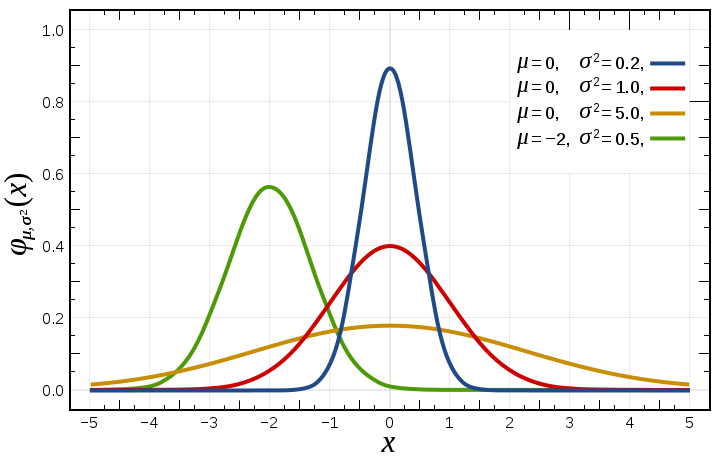
\includegraphics[width=\linewidth]{images/normal.png}
  		\caption{Normal distribution - variations in mean and SD}
  		\label{fig:normal dist.}
	\end{figure}

	Figure \ref{fig:normal dist.}.
	
	\item There's an empirical rule which states that 
	\begin{enumerate}
		\item 68.27\% data lies within 1 SD from the mean.
		\item 95.45\% data lies within 2 SD from the mean.
		\item 99.73\% data lies within 3 SD from the mean.				
	\end{enumerate}

	\begin{figure}
  		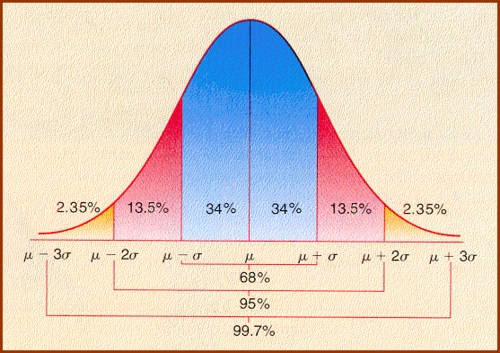
\includegraphics[width=\linewidth]{images/normalER.jpg}
  		\caption{Normal distribution - empirical rule}
  		\label{fig:normal er}
	\end{figure}	
	as shown in	Figure \ref{fig:normal er}.
	
	\item Example: Given mean weight of a person is 100kg with SD 10kg. Let us find the probability of his weight falling below 80kg.\\\\
	R code: pnorm(q = 80, mean = 100, sd = 10,lower.tail = T)\\ 
	lower.tail = T means $\le$\\\\
	Let us do it using $z-score$ where \mbox{\Large\(z=\frac{x-\mu}{\sigma}\)}\\\\
	
	z-score helps us interpret how far the value lies away from the mean in terms of standard deviation. We have already seen that most of the data in normal distribution lies within 3 standard deviation, left or right.\\
	\begin{center}
		{\Large\(z=\frac{80-100}{10}=-2\)}\\
	\end{center}
	Hence, data lies 2 SD away from mean in negative direction.\\ \\
	R code: pnorm(-2) results into same answer as with above R code.
	
\end{itemize}

\subsection{Log-normal}
\begin{itemize}
	\item A random variable whose logarithm is normally distributed is described with log-normal distribution.\\
	$\log(X)=W$\\
	or $x=e^{\mu + xz}$\\
	here,\\
	$z$ is a standard normal variable.
	\item PDF is given as 
	\mbox{\Large\(\frac{e\frac{-(ln(x)-\mu)^2}{2\sigma^2}}{x\sigma\sqrt{2}\pi}\)}
	\item Example: Given that the lifetime of a laptop follows a log-normal distribution with mean 12 hrs and sd 2 hours. Let us find the probability that its lifetime will be more than 50000 hrs.\\
	
	R code: 1 - plnorm(q = 50000, meanlog = 12, sdlog = 2)\\
	
\end{itemize}

\subsection{Negative exponential}

\begin{itemize}
	\item 
\end{itemize}

\end{document}